\documentclass[11pt,preprint]{elsarticle}

\usepackage{lmodern}
%%%% My spacing
\usepackage{setspace}
\setstretch{1.2}
\DeclareMathSizes{12}{14}{10}{10}

% Wrap around which gives all figures included the [H] command, or places it "here". This can be tedious to code in Rmarkdown.
\usepackage{float}
\let\origfigure\figure
\let\endorigfigure\endfigure
\renewenvironment{figure}[1][2] {
    \expandafter\origfigure\expandafter[H]
} {
    \endorigfigure
}

\let\origtable\table
\let\endorigtable\endtable
\renewenvironment{table}[1][2] {
    \expandafter\origtable\expandafter[H]
} {
    \endorigtable
}


\usepackage{ifxetex,ifluatex}
\usepackage{fixltx2e} % provides \textsubscript
\ifnum 0\ifxetex 1\fi\ifluatex 1\fi=0 % if pdftex
  \usepackage[T1]{fontenc}
  \usepackage[utf8]{inputenc}
\else % if luatex or xelatex
  \ifxetex
    \usepackage{mathspec}
    \usepackage{xltxtra,xunicode}
  \else
    \usepackage{fontspec}
  \fi
  \defaultfontfeatures{Mapping=tex-text,Scale=MatchLowercase}
  \newcommand{\euro}{€}
\fi

\usepackage{amssymb, amsmath, amsthm, amsfonts}

\def\bibsection{\section*{References}} %%% Make "References" appear before bibliography


\usepackage[numbers]{natbib}

\usepackage{longtable}
\usepackage[margin=2.3cm,bottom=2cm,top=2.5cm, includefoot]{geometry}
\usepackage{fancyhdr}
\usepackage[bottom, hang, flushmargin]{footmisc}
\usepackage{graphicx}
\numberwithin{equation}{section}
\numberwithin{figure}{section}
\numberwithin{table}{section}
\setlength{\parindent}{0cm}
\setlength{\parskip}{1.3ex plus 0.5ex minus 0.3ex}
\usepackage{textcomp}
\renewcommand{\headrulewidth}{0.2pt}
\renewcommand{\footrulewidth}{0.3pt}

\usepackage{array}
\newcolumntype{x}[1]{>{\centering\arraybackslash\hspace{0pt}}p{#1}}

%%%%  Remove the "preprint submitted to" part. Don't worry about this either, it just looks better without it:
\makeatletter
\def\ps@pprintTitle{%
  \let\@oddhead\@empty
  \let\@evenhead\@empty
  \let\@oddfoot\@empty
  \let\@evenfoot\@oddfoot
}
\makeatother

 \def\tightlist{} % This allows for subbullets!

\usepackage{hyperref}
\hypersetup{breaklinks=true,
            bookmarks=true,
            colorlinks=true,
            citecolor=blue,
            urlcolor=blue,
            linkcolor=blue,
            pdfborder={0 0 0}}


% The following packages allow huxtable to work:
\usepackage{siunitx}
\usepackage{multirow}
\usepackage{hhline}
\usepackage{calc}
\usepackage{tabularx}
\usepackage{booktabs}
\usepackage{caption}


\newenvironment{columns}[1][]{}{}

\newenvironment{column}[1]{\begin{minipage}{#1}\ignorespaces}{%
\end{minipage}
\ifhmode\unskip\fi
\aftergroup\useignorespacesandallpars}

\def\useignorespacesandallpars#1\ignorespaces\fi{%
#1\fi\ignorespacesandallpars}

\makeatletter
\def\ignorespacesandallpars{%
  \@ifnextchar\par
    {\expandafter\ignorespacesandallpars\@gobble}%
    {}%
}
\makeatother


% definitions for citeproc citations
\NewDocumentCommand\citeproctext{}{}
\NewDocumentCommand\citeproc{mm}{%
\href{\#cite.\detokenize{#1}}{#2}\nocite{#1}}

\makeatletter
% allow citations to break across lines
\let\@cite@ofmt\@firstofone
% avoid brackets around text for \cite:
\def\@biblabel#1{}
\def\@cite#1#2{{#1\if@tempswa , #2\fi}}
\makeatother
\newlength{\cslhangindent}
\setlength{\cslhangindent}{1.5em}
\newlength{\csllabelwidth}
\setlength{\csllabelwidth}{3em}
\newenvironment{CSLReferences}[2] % #1 hanging-indent, #2 entry-spacing
{\begin{list}{}{%
	\setlength{\itemindent}{0pt}
	\setlength{\leftmargin}{0pt}
	\setlength{\parsep}{0pt}
	% turn on hanging indent if param 1 is 1
	\ifodd #1
	\setlength{\leftmargin}{\cslhangindent}
	\setlength{\itemindent}{-1\cslhangindent}
	\fi
	% set entry spacing
	\setlength{\itemsep}{#2\baselineskip}}}
{\end{list}}

\usepackage{calc}
\newcommand{\CSLBlock}[1]{\hfill\break\parbox[t]{\linewidth}{\strut\ignorespaces#1\strut}}
\newcommand{\CSLLeftMargin}[1]{\parbox[t]{\csllabelwidth}{\strut#1\strut}}
\newcommand{\CSLRightInline}[1]{\parbox[t]{\linewidth - \csllabelwidth}{\strut#1\strut}}
\newcommand{\CSLIndent}[1]{\hspace{\cslhangindent}#1}


\urlstyle{same}  % don't use monospace font for urls
\setlength{\parindent}{0pt}
\setlength{\parskip}{6pt plus 2pt minus 1pt}
\setlength{\emergencystretch}{3em}  % prevent overfull lines
\setcounter{secnumdepth}{5}

%%% Use protect on footnotes to avoid problems with footnotes in titles
\let\rmarkdownfootnote\footnote%
\def\footnote{\protect\rmarkdownfootnote}
\IfFileExists{upquote.sty}{\usepackage{upquote}}{}

%%% Include extra packages specified by user
\usepackage{colortbl}
\usepackage{chngcntr}
\counterwithout{figure}{section}
\counterwithout{table}{section}\usepackage{booktabs}
\usepackage{longtable}
\usepackage{array}
\usepackage{multirow}
\usepackage{wrapfig}
\usepackage{float}
\usepackage{colortbl}
\usepackage{pdflscape}
\usepackage{tabu}
\usepackage{threeparttable}
\usepackage{threeparttablex}
\usepackage[normalem]{ulem}
\usepackage{makecell}
\usepackage{xcolor}

%%% Hard setting column skips for reports - this ensures greater consistency and control over the length settings in the document.
%% page layout
%% paragraphs
\setlength{\baselineskip}{12pt plus 0pt minus 0pt}
\setlength{\parskip}{12pt plus 0pt minus 0pt}
\setlength{\parindent}{0pt plus 0pt minus 0pt}
%% floats
\setlength{\floatsep}{12pt plus 0 pt minus 0pt}
\setlength{\textfloatsep}{20pt plus 0pt minus 0pt}
\setlength{\intextsep}{14pt plus 0pt minus 0pt}
\setlength{\dbltextfloatsep}{20pt plus 0pt minus 0pt}
\setlength{\dblfloatsep}{14pt plus 0pt minus 0pt}
%% maths
\setlength{\abovedisplayskip}{12pt plus 0pt minus 0pt}
\setlength{\belowdisplayskip}{12pt plus 0pt minus 0pt}
%% lists
\setlength{\topsep}{10pt plus 0pt minus 0pt}
\setlength{\partopsep}{3pt plus 0pt minus 0pt}
\setlength{\itemsep}{5pt plus 0pt minus 0pt}
\setlength{\labelsep}{8mm plus 0mm minus 0mm}
\setlength{\parsep}{\the\parskip}
\setlength{\listparindent}{\the\parindent}
%% verbatim
\setlength{\fboxsep}{5pt plus 0pt minus 0pt}



\begin{document}



\begin{frontmatter}  %

\title{Naming a Generation: How American Culture Writes Itself Into A
Cradle}

% Set to FALSE if wanting to remove title (for submission)




\author[Add1]{Diaz Sangeve}
\ead{24991422@sun.ac.za}





\address[Add1]{Stellenbosch University, Stellenbosch, South Africa}

\cortext[cor]{Corresponding author: Diaz Sangeve}

\begin{abstract}
\small{
A baby name is a small cultural record of the year a child was born.
Using the full state-level register of United States births from 1910 to
2014, together with the weekly Billboard Hot 100 since 1958 and a
catalogue of HBO titles and cast credits, this report does two things
for a creative agency. It measures how long popular names persist and
tests the agency's belief that persistence has weakened since the 1990s,
and it traces the sudden surges in naming back to the singers and screen
characters that set them off. Persistence has indeed loosened since
1990, at every horizon and most sharply for boys. The surges, meanwhile,
line up closely with hit records and popular premieres, and an event
study shows a name responding within a year or two of the moment that
created it.
}
\end{abstract}

\vspace{1cm}





\vspace{0.5cm}

\end{frontmatter}

\setcounter{footnote}{0}


\renewcommand{\contentsname}{Table of Contents}
{\tableofcontents}

%________________________
% Header and Footers
%%%%%%%%%%%%%%%%%%%%%%%%%%%%%%%%%
\pagestyle{fancy}
\chead{}
\rhead{}
\lfoot{}
\rfoot{\footnotesize Page \thepage}
\lhead{}
%\rfoot{\footnotesize Page \thepage } % "e.g. Page 2"
\cfoot{}

%\setlength\headheight{30pt}
%%%%%%%%%%%%%%%%%%%%%%%%%%%%%%%%%
%________________________

\headsep 35pt % So that header does not go over title




\section*{Naming a generation}\label{naming-a-generation}
\addcontentsline{toc}{section}{Naming a generation}

A baby name carries the fingerprint of its moment. It records what its
parents were listening to, watching and talking about in the year the
child arrived. With the full American birth register from 1910 to 2014,
alongside the Billboard Hot 100 and a catalogue of HBO titles, that
record can be read two ways. The first asks how durable a popular name
is, and whether durability has weakened. The second asks what lifts a
new name into use, and how quickly it answers.

\section*{Naming persistence and the 1990s
hypothesis}\label{naming-persistence-and-the-1990s-hypothesis}
\addcontentsline{toc}{section}{Naming persistence and the 1990s
hypothesis}

Persistence is measured by taking each year's 25 most popular names for
a gender and comparing their ranking to the same names one, two and
three years later. A Spearman rank correlation near one means the order
held, a lower value means the names moved or fell away.

\begin{figure}[H]

{\centering 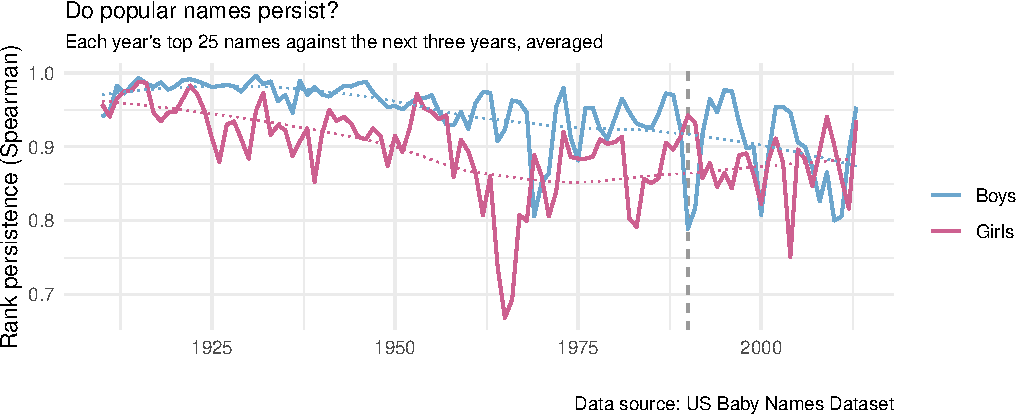
\includegraphics{Question2_files/figure-latex/fig-persist-1} 

}

\caption{Rank persistence of the top 25 names, each year against the next three. The dashed line marks 1990.}\label{fig:fig-persist}
\end{figure}

\begingroup\fontsize{9}{11}\selectfont

\begin{longtable}[t]{llrrr}
\caption{\label{tab:tab-persist}Mean rank persistence by gender and horizon, before and from 1990}\\
\toprule
Gender & Horizon & Pre-1990 & 1990 onward & Change\\
\midrule
Boys & 1-year & 0.981 & 0.950 & -0.031\\
Boys & 2-year & 0.958 & 0.891 & -0.067\\
Boys & 3-year & 0.934 & 0.836 & -0.098\\
Girls & 1-year & 0.952 & 0.937 & -0.014\\
Girls & 2-year & 0.900 & 0.868 & -0.032\\
\addlinespace
Girls & 3-year & 0.853 & 0.815 & -0.038\\
\bottomrule
\end{longtable}
\endgroup{}

\begin{itemize}
\tightlist
\item
  The agency's suspicion holds. Persistence falls after 1990 in every
  cell of the table, for both genders and at all three horizons.
\item
  The effect grows with distance. For boys the three-year persistence
  drops from 0.934 to 0.836, the largest fall in the table, so the
  further ahead you look the more a modern top name has moved.
\item
  Girls' names were always looser and slip less, from 0.853 to 0.815 at
  three years, so the change is real but gentler than for boys.
\item
  For the agency this means a name borrowed from today's culture is a
  weaker long-term bet than it would have been a generation ago, which
  is exactly what the surge analysis below explains.
\end{itemize}

\section*{When a name suddenly
arrives}\label{when-a-name-suddenly-arrives}
\addcontentsline{toc}{section}{When a name suddenly arrives}

The sharpest movements in naming are not drifts but spikes, and they can
be found directly in the data as large year-on-year jumps. The most
significant are striking, and many sit on a clear cultural event.

\begingroup\fontsize{9}{11}\selectfont

\begin{longtable}[t]{rlrrrl}
\caption{\label{tab:tab-surges}The ten sharpest year-on-year name surges, with the cause our datasets can attribute}\\
\toprule
Year & Name & Before & After & Times bigger & Cause\\
\midrule
1972 & Katina & 48 & 2726 & 56.8 & Other\\
1983 & Marquita & 96 & 2522 & 26.3 & Other\\
1966 & Audra & 36 & 865 & 24.0 & Other\\
1976 & Farrah & 36 & 813 & 22.6 & Other\\
1912 & Woodrow & 82 & 1826 & 22.3 & Other\\
\addlinespace
2001 & Nevaeh & 53 & 1179 & 22.2 & Other\\
1957 & Tammy & 204 & 4363 & 21.4 & Other\\
1954 & Sheree & 35 & 646 & 18.5 & Other\\
1992 & Devante & 86 & 1551 & 18.0 & Other\\
1994 & Aliyah & 43 & 707 & 16.4 & Other\\
\bottomrule
\end{longtable}
\endgroup{}

The supervisor's chart sets these out by name and year, sized by how
many babies took the name, with colour marking whether a singer or a
screen character drove it.

\begin{figure}[H]

{\centering 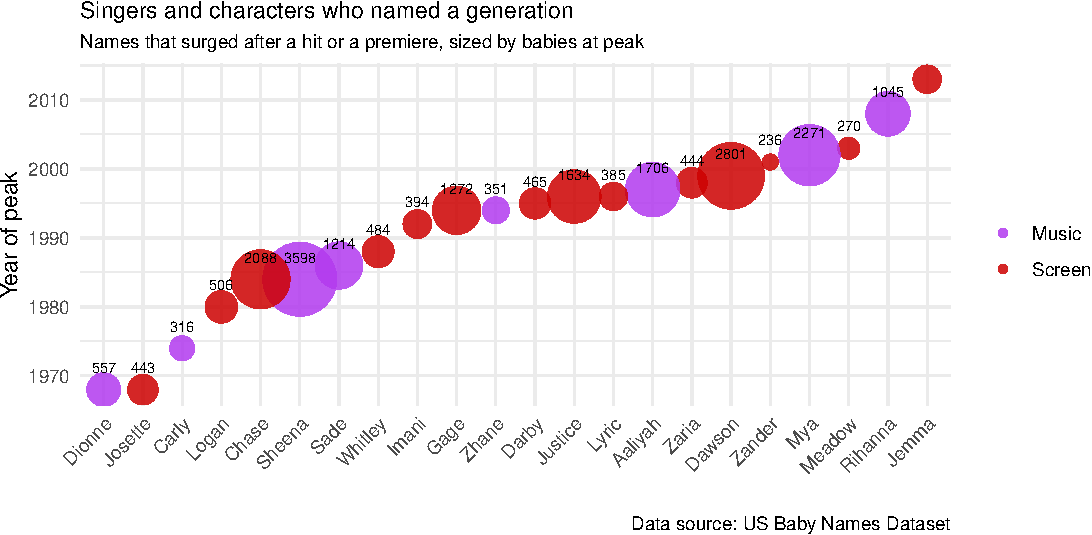
\includegraphics{Question2_files/figure-latex/fig-bubble-1} 

}

\caption{Names that surged after a hit record or a screen premiere, sized by babies at their peak.}\label{fig:fig-bubble}
\end{figure}

A surge is not the same as a lasting name. Plotting the largest surges
over their full life shows that most are fashions that fade within a
decade.

\begin{figure}[H]

{\centering 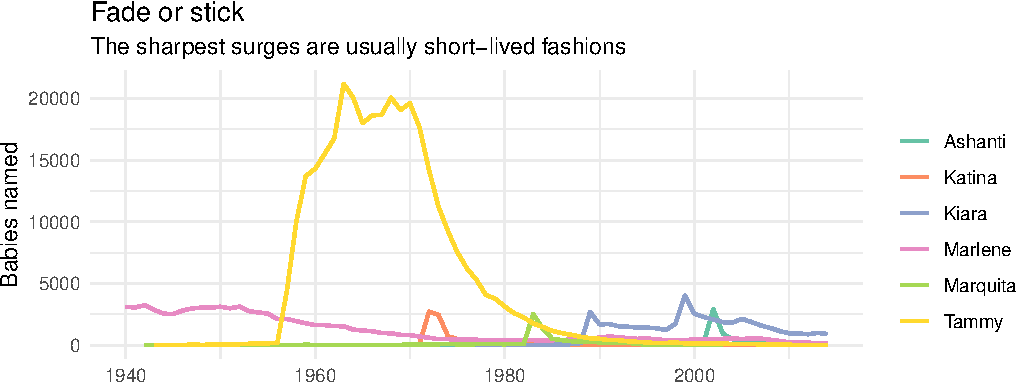
\includegraphics{Question2_files/figure-latex/fig-fade-1} 

}

\caption{The full trajectory of the sharpest surges. Most rise steeply and fall almost as fast.}\label{fig:fig-fade}
\end{figure}

\begin{itemize}
\tightlist
\item
  The surges are real and large. The sharpest, Katina in 1972,
  multiplied more than fifty times in a single year off the back of a
  television character.
\item
  Most of them fade. The same names that spike fastest tend to collapse
  within a few years, which is the surge-level reflection of the falling
  persistence in the previous section.
\item
  Colour ties cause to effect. Where our datasets reach the moment,
  screen characters and singers account for the surge, and the rest sit
  unexplained, waiting for the deeper look that follows.
\end{itemize}

A complementary view turns to the biggest names of the past century and
scales each to its own peak, so the shape of each rise and fall can be
read directly.

\begin{figure}[H]

{\centering 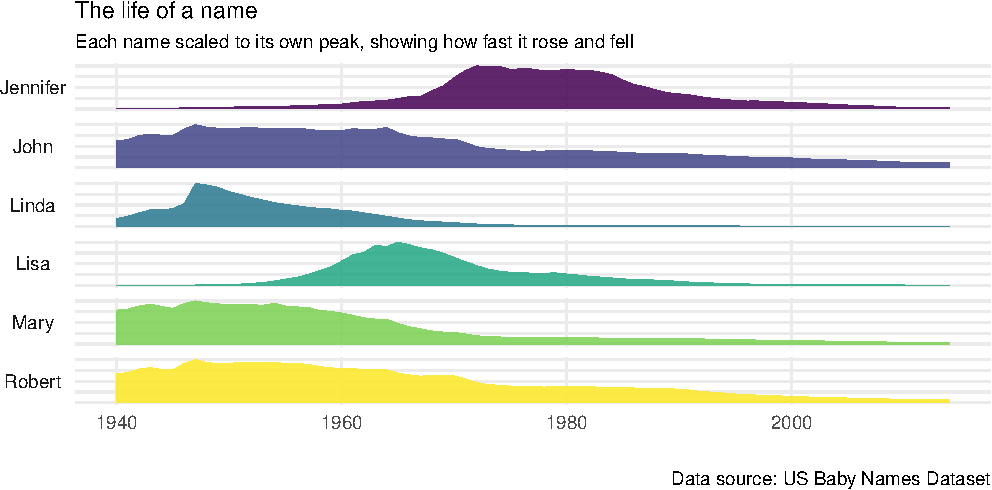
\includegraphics{Question2_files/figure-latex/fig-dist-1} 

}

\caption{The life of several culture-driven names, each scaled to its own peak.}\label{fig:fig-dist}
\end{figure}

\begin{itemize}
\tightlist
\item
  Even the giants are temporary. Linda and Lisa tower over their decades
  and then all but vanish, each now a fraction of a percent of its own
  peak.
\item
  This is the persistence finding seen one name at a time. No name holds
  the top for long, the same impermanence the Spearman series measured
  in aggregate.
\end{itemize}

\section*{The sound and the screen}\label{the-sound-and-the-screen}
\addcontentsline{toc}{section}{The sound and the screen}

The surge view points at music and television without proving them. The
Billboard and HBO datasets let us test both directly, by reading the
first name of every charting act and every screen character and asking
whether babies followed.

\subsection*{Named after the charts}\label{named-after-the-charts}
\addcontentsline{toc}{subsection}{Named after the charts}

\begingroup\fontsize{9}{11}\selectfont

\begin{longtable}[t]{llrrrr}
\caption{\label{tab:tab-billboard}Singers whose first name surged in babies after they first reached the Billboard top ten}\\
\toprule
Name & Artist & First charted & Before & Peak & Times bigger\\
\midrule
Sade & Sade & 1985 & 0 & 1214 & 1214.0\\
Rihanna & Rihanna & 2005 & 0 & 1045 & 1045.0\\
Zhane & Zhane & 1993 & 0 & 351 & 351.0\\
Aaliyah & Aaliyah & 1994 & 5 & 1706 & 284.3\\
Carly & Carly Simon & 1971 & 5 & 316 & 52.7\\
\addlinespace
Sheena & Sheena Easton & 1981 & 90 & 3598 & 39.7\\
Dionne & Dionne Warwick & 1964 & 18 & 557 & 29.8\\
Mya & Mya \& Sisqo & 1998 & 101 & 2271 & 22.3\\
\bottomrule
\end{longtable}
\endgroup{}

\begin{figure}[H]

{\centering 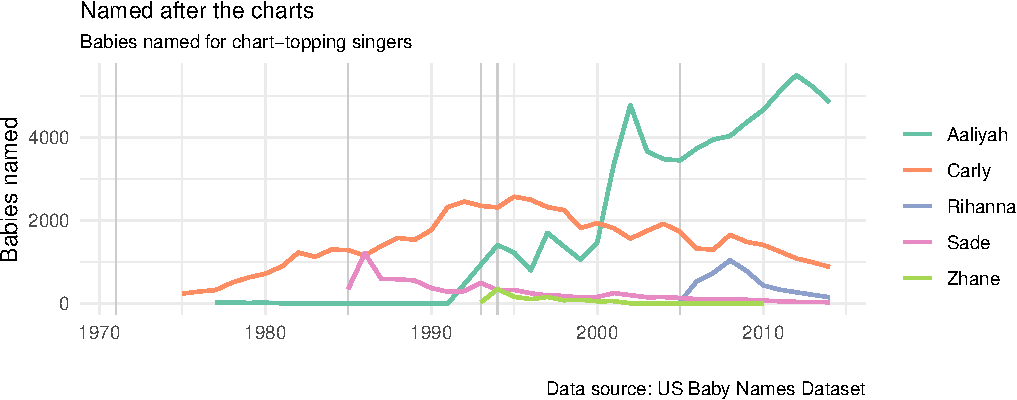
\includegraphics{Question2_files/figure-latex/fig-billboard-1} 

}

\caption{Naming after the charts. Dotted lines mark the year each act first reached the top ten.}\label{fig:fig-billboard}
\end{figure}

\begin{itemize}
\tightlist
\item
  The chart all but creates names. Sade and Rihanna barely existed
  before their first hit and then ran into the thousands, with Aaliyah
  close behind, while Zhane and Carly show the same shape on a smaller
  scale.
\item
  The brief's Whitney example is the same mechanism in a milder form.
  Whitney was already a known name, 1,547 births in 1982, and Houston
  lifted it more than sixfold to 9,719 by 1986. Because it was already
  common it sits just outside a table built to surface names the charts
  created from almost nothing.
\end{itemize}

\subsection*{Named after the screen}\label{named-after-the-screen}
\addcontentsline{toc}{subsection}{Named after the screen}

\begingroup\fontsize{9}{11}\selectfont

\begin{longtable}[t]{llrrrr}
\caption{\label{tab:tab-hbo}Screen characters whose first name surged in babies after the title appeared}\\
\toprule
Name & Title & Released & Score & Peak & Times bigger\\
\midrule
Whitley & A Different World & 1987 & 6.7 & 484 & 484.0\\
Zaria & The Parent 'Hood & 1995 & 6.4 & 444 & 444.0\\
Meadow & The Sopranos & 1999 & 8.5 & 270 & 270.0\\
Zander & Starship Troopers & 1997 & 7.0 & 236 & 236.0\\
Lyric & Jason's Lyric & 1994 & 6.6 & 385 & 64.2\\
\addlinespace
Justice & The Pelican Brief & 1993 & 6.6 & 1634 & 29.5\\
Imani & Coming to America & 1988 & 6.8 & 394 & 28.1\\
Gage & Tales from the Darkside: The Movie & 1990 & 6.1 & 1272 & 25.6\\
\bottomrule
\end{longtable}
\endgroup{}

\begin{figure}[H]

{\centering 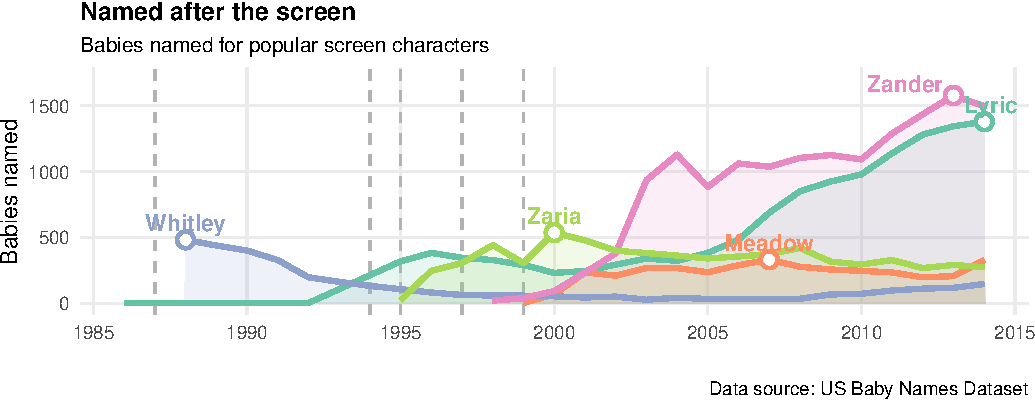
\includegraphics{Question2_files/figure-latex/fig-hbo-1} 

}

\caption{Naming after the screen. Dotted lines mark each title's release year.}\label{fig:fig-hbo}
\end{figure}

\begin{itemize}
\tightlist
\item
  Characters travel from the screen into the register. Meadow rises
  after The Sopranos, Whitley after A Different World, and Imani after
  Coming to America, each within a year or two of the title appearing.
\item
  The supervisor's Katina is the same mechanism a generation earlier, a
  character name that arrived the moment the show did.
\item
  A caution on the source. The HBO catalogue includes films streamed on
  the service, not only its own productions, so entries like Zander or
  Lyric are candidate associations rather than proven causes. The
  strongest cases are the distinctive names tied to genuinely popular,
  character-led shows.
\end{itemize}

\subsection*{How fast a culture names a
child}\label{how-fast-a-culture-names-a-child}
\addcontentsline{toc}{subsection}{How fast a culture names a child}

Pooling every matched name and lining each one up on the year its
trigger landed gives an event study, the average naming response to a
hit or a premiere. Each name is scaled to its own peak, so the curve
reads as the share of a name's eventual high point reached at each step
from the event.

\begin{figure}[H]

{\centering 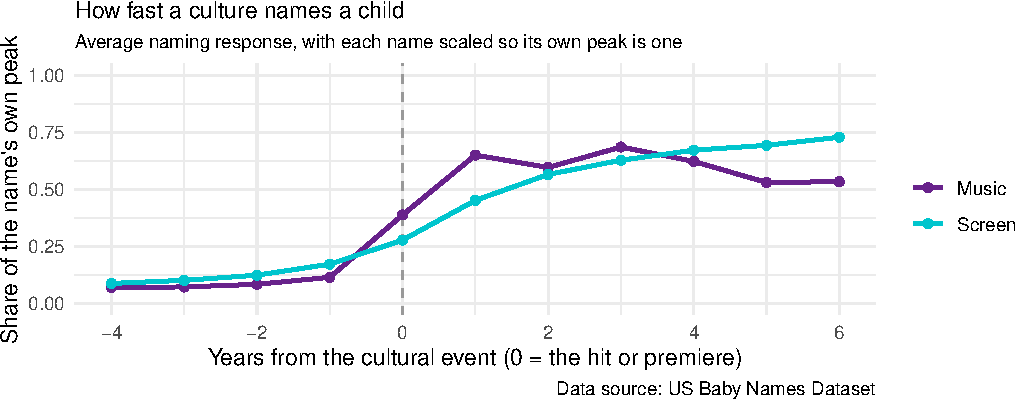
\includegraphics{Question2_files/figure-latex/fig-event-1} 

}

\caption{Average naming response around the cultural event, music against screen.}\label{fig:fig-event}
\end{figure}

\begin{itemize}
\tightlist
\item
  The event is the hinge. Both music and screen names sit near a tenth
  of their peak in the years before, then turn upward the moment the hit
  or premiere lands.
\item
  Music is fast and front-loaded. A charting name reaches roughly two
  thirds of its peak within a single year and tops out inside three,
  matching a song's instant, saturating reach before it fades.
\item
  Screen is slow and durable. A character name climbs gently and is
  still rising six years on, which fits a show that builds its audience
  season by season.
\item
  Either way the response is quick. Within a year or two of the moment
  the name is already well on its way, so naming tracks culture almost
  in real time.
\end{itemize}

\section*{What names follow}\label{what-names-follow}
\addcontentsline{toc}{section}{What names follow}

Two findings sit together. Popular names hold their place less firmly
than they once did, especially for boys and especially since 1990, so
any name the agency borrows from culture should be treated as a moving
target. And the thing that moves it is close cultural reach, the singers
on the charts and the characters on the screen, whose names enter the
register within a year or two and then, more often than not, recede
again. A name is a fashion with a date stamp, and the data shows both
the stamp and the fading ink.

\bibliography{Tex/ref}





\end{document}
